\documentclass[11pt, oneside]{article} 
\usepackage{geometry}
\geometry{letterpaper} 
\usepackage{graphicx}
	
\usepackage{amssymb}
\usepackage{amsmath}
\usepackage{parskip}
\usepackage{color}
\usepackage{hyperref}

\graphicspath{{/Users/telliott_admin/Dropbox/Tex/png/}}
% \begin{center} 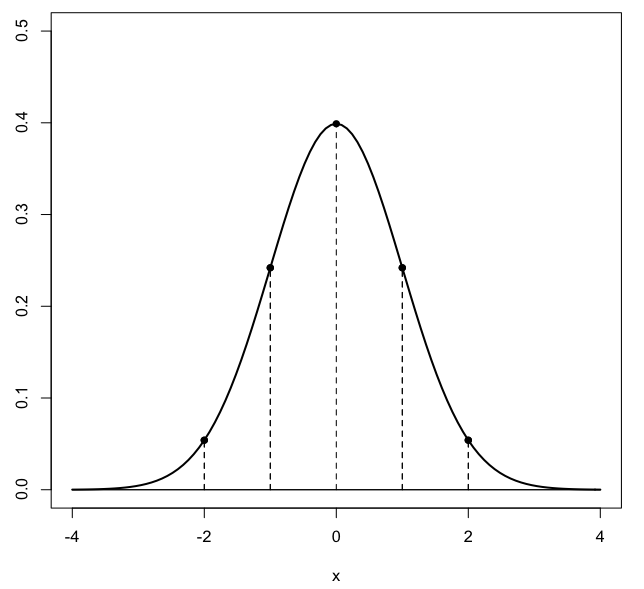
\includegraphics [scale=0.4] {gauss3.png} \end{center}

\title{Modular arithmetic}
\date{}

\begin{document}
\maketitle
\Large

Modular arithmetic is all of

\begin{itemize}
	\item addition
	\item multiplication
	\item subtraction
	\item division
\end{itemize}

with integers, all carried out modulo (or mod) some integer $n$. 

The rule is to keep the remainder after dividing by the modulus.  This called the "mod" operation and is often symbolized \% as well as mod.

\subsection*{Addition}

Here is an addition table for $n = 4$:

\newpage

\begin{verbatim}
    0  1  2  3  
   ------------
0 | 0  1  2  3
1 | 1  2  3  0
2 | 2  3  0  1
3 | 3  0  1  2
\end{verbatim}

Example:  $3 + 2 = 5  \text{ mod } 4 = 1$

Since $36  \text{ mod } 7 = 1$ and $15 \text{ mod } 7 = 1$ as well, it follows that
\[ 36 = 15 \text{ mod } 7 = 1 \]

These two numbers are also equal to $8, 22, 29$ and so on.

Alternatively, we may write
\[ 36 = 1 (\text{ mod } 7) \]

\subsection*{Multiplication}

Consider multiplication mod $6$ (first table) and mod $7$ (second table)
\begin{verbatim}
  6
  1  |  0  1  2  3  4  5
  2  |  0  2  4  0  2  4
  3  |  0  3  0  3  0  3
  4  |  0  4  2  0  4  2
  5  |  0  5  4  3  2  1

  7
  1  |  0  1  2  3  4  5  6
  2  |  0  2  4  6  1  3  5
  3  |  0  3  6  2  5  1  4
  4  |  0  4  1  5  2  6  3
  5  |  0  5  3  1  6  4  2
  6  |  0  6  5  4  3  2  1
\end{verbatim}

The tables were constructed by standard multiplication, followed by the indicated mod operation.

Looking at the contents of the tables, notice that for $n = 6$, only the rows with multiplications of $1$ and $5$ generated all the integers less than $6$.  This is a common pattern, it's always true that $1$ and $n-1$ generate all the values $< n$.  

That's because

\[ a \times 1 + a \times (n-1) = 0 \ (\text{mod} \ n) \]

and that's because

\[ a \times 1 + a \times (n-1)) = a + na - a = na = 0 \ (\text{ mod n }) \]

For $n = 7$, every number generated all the other ones.

\textbf{Since all integers smaller than n are generated from each starting integer in the special case, a unique result must be produced for each multiplication.}

That statement is worth parsing carefully.

If a number, multiplied by all the elements of the field generates all the elements of the field, then at least one of those results must be equal to $1$.  

The two multiplicands with this property are called multiplicative inverses. 

Each row contains all possible values $< n$ if $n$ is prime.

An interesting case is one where n is not prime, yet certain integers other than $1$ and $n-1$ generate all the integers smaller than $n$.  

It turns out that this happens when the smaller number is co-prime with $n$ (they have no common factors other than $1$).

So for example, here is the multiplication table for $n = 8$ where all integers smaller than $8$ are generated by $3$ and $5$:

\begin{verbatim}
8
  1  |  0  1  2  3  4  5  6  7
  2  |  0  2  4  6  0  2  4  6
  3  |  0  3  6  1  4  7  2  5
  4  |  0  4  0  4  0  4  0  4
  5  |  0  5  2  7  4  1  6  3
  6  |  0  6  4  2  0  6  4  2
  7  |  0  7  6  5  4  3  2  1
\end{verbatim}

$6$ is not co-prime to $8$ because they share the common factor $2$, whereas $3$ and $5$ are co-prime.  So both $3$ and $5$ are their own multiplicative inverses.

\subsection*{Powers}

With $n = 7$, consider the powers of each $ i < 7$:

\begin{verbatim}
    1  2  3  4  5  6
   ---------------------
1 | 1  2  3  4  5  6
2 | 2  4  1  2  4  1
3 | 3  2  6  4  5  1
4 | 4  2  1  4  2  1
5 | 5  4  6  2  3  1  
6 | 6  1  6  1  6  1
\end{verbatim}

This table can be a challenge to construct.  I wrote a script to help with the calculations the first time through. 

We discover that the powers of $3$ and $5$ (but not $2,4,6$) give all the integers $<7$.  

These two (but not only these two) have the property that

- $3^{n-1} = 3^6 = 1 \ \ \ \ 3^n = 3$

- $5^{n-1} = 5^6 = 1 \ \ \ \ 5^n = 5$

This is what wikipedia means when they talk about the "q - 1 power of unity".

\subsection*{Take the modulus at each step}

\begin{quote}...in any expression involving +, $-$, $\times$ and positive integer exponents (that is, any "polynomial''), if individual terms are replaced by other terms that are congruent to them modulo $n$, the resulting expression is congruent to the original."\end{quote}

Because of distributivity, a mod can be taken any time.  Example:
\[ 5 + 5 + 5 + 5  + 5 + 5 = 30 \text{ mod 7 } = 2 \]

Taking the mod at every other step:
\[ 5 + 5 = 10 \text{ mod 7 } = 3 \]
\[ 5 + 5 + 5 + 5 + 5 + 5 = 3 + 3 + 3 = 9 \text{ mod 7 } = 2 \]

This keeps the numbers small and it works because if $z = x \times y$ then

\[ z  \text{ mod } n = (x  \text{ mod } n) * (y  \text{ mod } n) \]

Every integer is equal to an integer $q$ times $ n$, which is divided evenly by $n$, plus a remainder $r < n$.  So

\[ x = qn + r \]
\[ y = q'n + r' \]
and then
\[ x \times y = (qn \times q'n) + (qn \times r') + (r \times q'n) + (r \times r') \]

The only term on the right which is not evenly divisible by $n$ is the last one.  Thus

\[ (x \times y)  \text{ mod } n = (r \times r')  \text{ mod } n \]

So, for example 

\[ 5^2 = 25 = 4 \text{ mod } 7 \]

and 
\[ 5^4 = (5^2)^2 = 4^2 = 2 (\text{ mod } 7) \]

Another example:  in the row

\begin{verbatim}
5 | 5  4  6  2  3  1
\end{verbatim}

The value at position 5 is equal to the product of the values at positions 2 and 3:  $4 \times 6 = 24 = 3 \ (\text{ mod } 7)$.

\subsection*{Division}

Consider multiplication mod n = 7 again:

\begin{verbatim}
  7
  1  |  0  1  2  3  4  5  6
  2  |  0  2  4  6  1  3  5
  3  |  0  3  6  2  5  1  4
  4  |  0  4  1  5  2  6  3
  5  |  0  5  3  1  6  4  2
  6  |  0  6  5  4  3  2  1
\end{verbatim}

Since $2 \times 4 = 1$ (mod 7), 4 and 2 are multiplicative inverses, similarly $(3,5)$ and $(6,6)$ as well as $(1,1)$.  This allows us to say that division by $q$ is the same as multiplication by the multiplicative inverse of $q$.  So
\[  5 / 4 = 2 * 5 = 3 (\text{ mod } 7) \]

\end{document}